\documentclass[conf]{new-aiaa}
%\documentclass[journal]{new-aiaa} for journal papers
\usepackage[utf8]{inputenc}

\usepackage{graphicx}
\usepackage{amsmath}
\usepackage[version=4]{mhchem}
\usepackage{siunitx}
\usepackage{longtable,tabularx}
\usepackage{multirow}

\setlength\LTleft{0pt} 

\title{Proposal for the Geological and Atmospheric Data Expansion of Titan}

\author{Brig Goodwin\footnote{Astrodynamics Specialist.}, Blake Johnson\footnote{Science Specialist}, Sung Jae Kim\footnote{Propulsion Specialist}, and Thad Tucker\footnote{Electronics Specialist}}
\affil{College of Engineering, University of Oklahoma, Norman, Ok, 73019}


\begin{document}

\maketitle

\section{Introduction}
\subsection{Proposal for the mission}
We propose sending a rover to Saturn's moon Titan to measure surface samples and perform topical analysis on different geological areas. We will identify the chemical makeup of the topical ice/minerals.  In order to obtain a general overview, we will take multiple samples from different "zones" spaced several miles apart.\\
\par In addition to taking the above measurements, we will determine the age of underlying ice/minerals. We will then be able to assemble a better understanding of Titan's overall makeup. We will release a deep space satellite in a highly eccentric orbit around Titan while in orbit. The satellite will establish a link with the rover on Titan and with the home base on Earth. This allows smooth communication with Titan and the Deep Space Satellite Network. It will also provide overall communication with all systems during the duration of the mission and missions to follow.\\
\par Titan is the only known satellite orbiting a body in the solar system to have an atmosphere. Furthermore, the atmosphere is $97\%$ nitrogen compared to Earth's $78\%$ Nitrogen atmosphere\cite{NASA}. Titan is the only nitrogen-rich atmosphere in the solar system other than Earth's atmosphere. Given the similarities between Earth's atmosphere and Titan's atmosphere, studying the atmosphere and comparing the two atmospheres will help us better understand our own atmosphere.  This is important for the continued human development on Earth, the possibilities of improving the Earth's atmosphere and repairing damages caused by global warming, and our ongoing understanding of extraterrestrial atmospheres to better expand our knowledge of our Universe.

\subsection{Motivation for the mission}
\par Titan and Earth have many similarities with each other, most notably their nitrogen-heavy atmospheres. However due to its dense atmosphere, very little is currently known about Titan.  Having the opportunity to land and study Titan's geological makeup up-close provides many opportunities and could lead toward discovering answers to questions we have regarding our own planet.\\
\par Since we, as a species, are working towards colonizing Mars and becoming an interplanetary species, we must continue to expand our foothold in the solar system.  Titan will be the next logical location for us to begin studying now that we have rovers on Mars.
\subsection{Benefits of the mission}
\par There are several potential benefits to the exploration of Titan.  Primarily, by gaining a better understanding of Titan's atmosphere and atmospheric conditions, we potentially could better understand our own atmosphere. With global warming being such a highly debated topic politically, we may better understand how to combat global warming in the future.  With more science and data collected, we can also have a better understanding of the consequences of carbon emissions.  We might be able to obtain a healthy substitute for carbon emissions. In any of these cases, gaining a better understanding of Titan's atmosphere will benefit the human race here on Earth.\\
\par Titan's surface is believed to be comprised of solid-liquid water. The search for water in the Universe is vital to the exploration of extraterrestrial life. Analyzing the water on Titan, much like we did on Mars, might provide us with evidence of microscopic organisms off the planet and help determine if life can exist outside our atmosphere.\\
\par Titan also has rivers and lakes of liquid ethane and methane.  This is the only known object in the solar system other than Earth to have liquid rivers and lakes.  This is important to study to help us better understand our own planet's makeup, as well as give us more information on other planets to use during our exploration.\\
\par We will also be placing a satellite in orbit around Saturn.  This is a long-term satellite designed to be used for future space explorations.  It will not only help us accomplish our mission but will also help save time and money on future missions.

\section{Astrodynamics}

\subsection{Introduction}
This report outlines the estimated $\Delta v$ required for a spacecraft to reach Titan, Saturn's largest moon, from a circular parking orbit around Earth. The Huygens probe is the only craft to land on Titan, which was carried to the distant moon via NASA's Cassini flyby mission in 2005. The Cassini mission used a total of four gravity assists to reach Saturn, including two from Venus, one from Earth, and another from Jupiter. This complex mission design allowed it to visit multiple planets with superior efficiency. In this study, we evaluate the case of a standard interplanetary Hohmann transfer maneuver to land a spacecraft on Titan. Rather than improving efficiency via gravity assist, the novelty of our mission design is to take advantage of Titan's thick atmosphere and land via aerobraking. We demonstrate that a significant amount of $\Delta v$ could be spared by this method as opposed to achieving a capture orbit by propellant only. 
%%%%%%%%%%%%%%%%%%%%%%%%%%%%%%%%%%%%%%%%%%%%%%%%%%%%%%%%%%%%%%%%%%%%%%%%%%%%%%%%%%%%%%%%%%%%%%%%%%%%%%%%%%%%%%%%%%%%%%%%%%%%

%%%%%%%%%%%%%%%%%%%%%%%%%%%%%%%%%%%%%%%%%%%%%%%%%%%%%%%%%%%%%%%%%%%%%%%%%%%%%%%%%%%%%%%%%%%%%%%%%%%%%%%%%%%%%%%%%%%%%%%%%%%%
\subsubsection{Planetary Data}

\begin{table}[htbp]
\centering
\begin{tabular}{| c c c c c c |}
\hline
Body & $\mu(km^3/s^2)$ & $r (km)$ & $R (km)$ & $P (days)$ & $m (kg)$ \\
\hline
Earth & $398,600$ & $6,378$ & $149.6 \times 10^6$ & $365.256$ & $5.974 \times 10^{24}$ \\
Saturn & $37,931,187$ & $60,270$ & $1.433 \times 10^9$ & $10760.4$ & $568.5 \times 10^{24}$ \\
Titan & $8,978$ & $2,575$ & *$1.2 \times 10^6$ & *$15.92$ & $1.345 \times 10^{23}$ \\
Sun & $132,712,440,018$ & $696,000$ & $-$ & $-$ & $1.989 \times 10^{30}$ \\
\hline
\end{tabular}
\caption{\label{tab:widgets}Planetary data for bodies relevant to mission. *With respect to Saturn.}
\end{table}
%%%%%%%%%%%%%%%%%%%%%%%%%%%%%%%%%%%%%%%%%%%%%%%%%%%%%%%%%%%%%%%%%%%%%%%%%%%%%%%%%%%%%%%%%%%%%%%%%%%%%%%%%%%%%%%%%%%%%%%%%%%%

%%%%%%%%%%%%%%%%%%%%%%%%%%%%%%%%%%%%%%%%%%%%%%%%%%%%%%%%%%%%%%%%%%%%%%%%%%%%%%%%%%%%%%%%%%%%%%%%%%%%%%%%%%%%%%%%%%%%%%%%%%%%
\subsection{Interplanetary Hohmann Transfer}
For these calculations, we make the fundamental assumption that all orbits are circular and co-planar. Parameters for Earth are labelled by the subscript 1, Saturn by 2, and Titan by 3. Values for the sun as the central body are labelled explicitly, and numerical values for each particular variable are given in Table 1 along with their corresponding units.
%%%%%%%%%%%%%%%%%%%%%%%%%%%%%%%%%%%%%%%%%%%%%%%%%%%%%%%%%%%%%%%%%%%%%%%%%%%%%%%%%%%%%%%%%%%%%%%%%%%%%%%%%%%%%%%%%%%%%%%%%%%%

%%%%%%%%%%%%%%%%%%%%%%%%%%%%%%%%%%%%%%%%%%%%%%%%%%%%%%%%%%%%%%%%%%%%%%%%%%%%%%%%%%%%%%%%%%%%%%%%%%%%%%%%%%%%%%%%%%%%%%%%%%%%
\subsubsection{Heliocentric Trajectory}

Here we find $\Delta v$ required to execute a Hohmann transfer from an Earth orbit to a Saturn orbit. Note that this calculation has no dependence on the bodies of Earth and Saturn themselves and depends only on the orbital radii. The velocity of a body in circular heliocentric orbit at Earth's radius R is

\begin{equation}
    v_1=\sqrt{\frac{ \mu_{\text{sun}} }{ R_ 1 }} = 29.7845 \ km/s.
\end{equation}

and the departure velocity required to raise apoapsis to the radius R of Saturn is

\begin{equation}
    v_D = \sqrt{2\mu_{\text{sun}}}\sqrt{\frac{R_ 2}{R_ 1(R_ 1+R_ 2)}} = 40.0814 \ km/s.
\end{equation}

Therefore the $\Delta v$ required for the first burn is

\begin{equation}
\Delta \!\ v_1 = v_D - v_ 1 = \sqrt{\frac{\mu_{\text{sun}}}{R_1}}(\sqrt{\frac{2R_ 2}{R_ 1 +R_ 2}}-1) = 10.2969 \ km/s
\end{equation}

Now, the velocity of a body in circular orbit around the sun at Saturn's distance is

\begin{equation}
v_ 2=\sqrt{\frac{ \mu_{\text{sun}} }{ R_ 2\ }} = 9.62349 \ km/s
\end{equation}

and velocity of a body at the apoapsis of the transfer ellipse created from the first burn is

\begin{equation}
v_A = \sqrt{2\mu_{\text{sun}}}\sqrt{\frac{R_ 1}{R_ 2(R_ 1+R_ 2)}} = 4.18435 \ km/s.
\end{equation}

Therefore the $\Delta v$ required on the second burn to circularize and bring perigee up to apogee is

\begin{equation}
\Delta \!\ v_2 = v_A - v_ 2 = \sqrt{\frac{\mu_{\text{sun}}}{R_ 2}}(1 - \sqrt{\frac{2R_ 1}{R_ 1 +R_ 2}}) = 5.43914 \ km/s.
\end{equation}

So for the total $\Delta v$ of both maneuvers, we have

\begin{equation}
\Delta v_{\text{tot}} = \Delta v_1 + \Delta v_2 = 15.736 \ km/s.
\end{equation}
%%%%%%%%%%%%%%%%%%%%%%%%%%%%%%%%%%%%%%%%%%%%%%%%%%%%%%%%%%%%%%%%%%%%%%%%%%%%%%%%%%%%%%%%%%%%%%%%%%%%%%%%%%%%%%%%%%%%%%%%%%%%

%%%%%%%%%%%%%%%%%%%%%%%%%%%%%%%%%%%%%%%%%%%%%%%%%%%%%%%%%%%%%%%%%%%%%%%%%%%%%%%%%%%%%%%%%%%%%%%%%%%%%%%%%%%%%%%%%%%%%%%%%%%%
\subsubsection{Phase Angle}

We now consider the required phase angle for rendezvous between bodies at each circular orbit. First, we find the semi-major axis of the transfer ellipse:

\begin{equation}
a = \frac{1}{2}(R_ 1 + R_ 2) = 7.913 \times 10^8 \ km.
\end{equation}

Time of flight along the elliptical trajectory is half of the orbital period:

\begin{equation}
t = \frac{\pi}{\sqrt{\mu_{\text{sun}}}}a^{3/2} = 1.92 \times 10^8 \text{s} \ (2221.73 \ \text{days, or} \ 6.083 \ \text{years.})
\end{equation}

Phase angle between bodies at departure can then be found using angular velocity $\omega$ (rad/day): 

\begin{equation}
\phi_0 = \pi -\omega_2 t = 1.8443 \ \text {rad} = 105.67^{\circ}.
\end{equation}

\begin{figure}[htp]
    \centering
    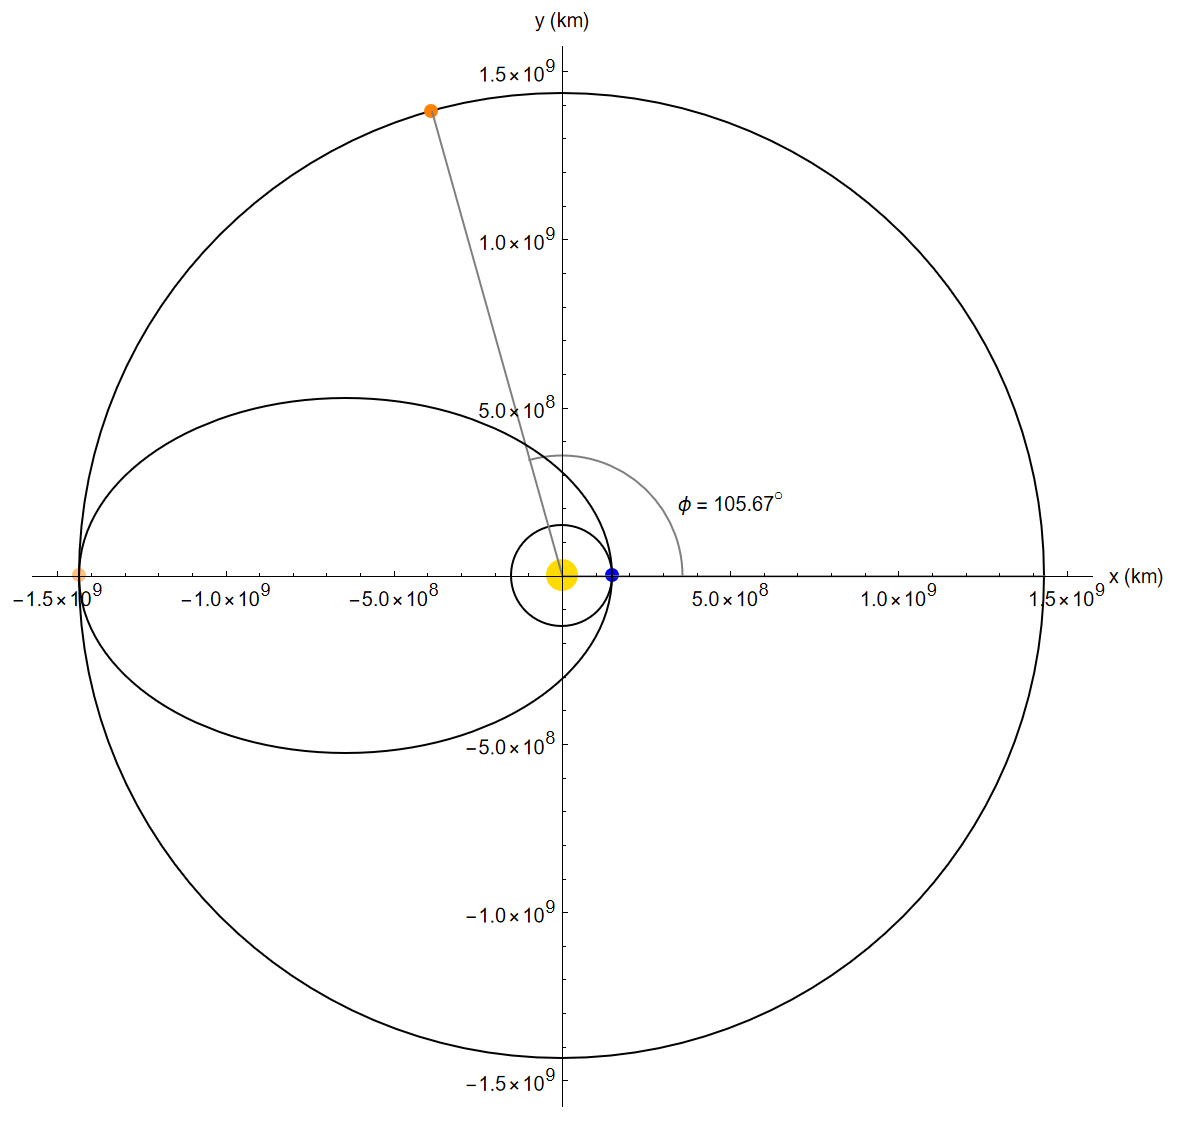
\includegraphics[width=7.5cm]{Project Figure 1.png}
    \caption{Model for Earth to Saturn rendezvous trajectory with phase angle $\phi$.}
\end{figure}
%%%%%%%%%%%%%%%%%%%%%%%%%%%%%%%%%%%%%%%%%%%%%%%%%%%%%%%%%%%%%%%%%%%%%%%%%%%%%%%%%%%%%%%%%%%%%%%%%%%%%%%%%%%%%%%%%%%%%%%%%%%%

%%%%%%%%%%%%%%%%%%%%%%%%%%%%%%%%%%%%%%%%%%%%%%%%%%%%%%%%%%%%%%%%%%%%%%%%%%%%%%%%%%%%%%%%%%%%%%%%%%%%%%%%%%%%%%%%%%%%%%%%%%%%
\subsection{Patched Conic Approximation}

We can obtain a more accurate $\Delta v$ estimate by assuming an initial parked orbit around Earth achieved by the first stage of the rocket. For our mission design, we assume a circular orbit at 600 km altitude from the surface. The patched conic method considers velocities relative to whichever body is gravitationally dominant at the spacecraft's current position. This means the elliptical heliocentric trajectory previously calculated remains relevant for most of the mission, but is patched together with hyperbolas at Earth and Saturn when the spacecraft is within their respective sphere of influence (SOI).

\subsubsection{Earth Departure}

The spacecraft's exit velocity at the boundary of Earth's sphere of influence frame will be equal to the velocity gained after the first burn $\delta v_1$:

\begin{equation}
v_{\infty 1}=\sqrt{\frac{\mu_{\text{sun}}}{R_ 1}}(\sqrt{\frac{2R_2}{R_ 1 +R_ 2}}-1) = 10.2969 \ km/s.
\end{equation}

Periapsis velocity assuming an initial parking orbit height of 600 km would be

\begin{equation}
v_{p1} =\sqrt{v_ {\infty 1}^2 + \frac{2\mu_1}{r_{p1}}} = 14.8415 \ km/s
\end{equation}

and the parking orbit velocity before the burn is

\begin{equation}
v_{c1} = \sqrt{\frac{\mu_{1}}{r_{p1}}} = 7.55794 \ km/s,
\end{equation}

so the $\Delta v$ required to leave Earth's sphere of influence is

\begin{equation}
\Delta \!\ v_{\inf 1} = v_{p1} - v_{c1} = v_{c1} (\sqrt{2+(\frac{v_{\infty 1}}{v_{c1}})^2}-1) = 7.28358 \ km/s.
\end{equation}

The departure angle for the first burn can then be found as

\begin{equation}
\beta = \cos^{-1}[(1+\frac{r_{p1} v_ {\infty 1}^2}{\mu_1})^{-1}] = 1.213 \ \text {rad} = 69.5^{\circ}.
\end{equation}

\begin{figure}[htp]
    \centering
    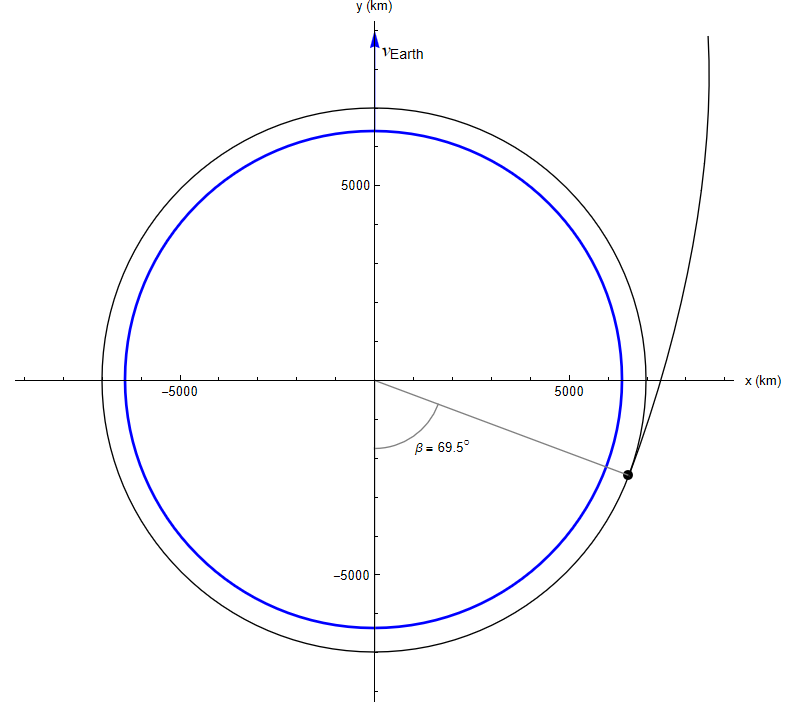
\includegraphics[width=7.5cm]{Project Figure 2.png}
    \caption{Craft(Black) in a 600km circular orbit over Earth(Blue) with departure angle $\beta$ for transfer burn and hyperbolic trajectory.}
\end{figure}
%%%%%%%%%%%%%%%%%%%%%%%%%%%%%%%%%%%%%%%%%%%%%%%%%%%%%%%%%%%%%%%%%%%%%%%%%%%%%%%%%%%%%%%%%%%%%%%%%%%%%%%%%%%%%%%%%%%%%%%%%%%%

%%%%%%%%%%%%%%%%%%%%%%%%%%%%%%%%%%%%%%%%%%%%%%%%%%%%%%%%%%%%%%%%%%%%%%%%%%%%%%%%%%%%%%%%%%%%%%%%%%%%%%%%%%%%%%%%%%%%%%%%%%%%
\subsubsection{Saturn Rendezvous}

Arrival velocity at the boundary of Saturn's sphere of influence will be:

\begin{equation}
v_{\infty 2} = v_ 2 - v_A = 5.43914 \ km/s.
\end{equation}

Velocity at nearest approach with $r_p$ being the same orbital distance as Titan $R_3$ is then

\begin{equation}
v_{p2} =\sqrt{v_ {\infty 2}^2 + \frac{2\mu_2}{R_3}} = 9.63343\ km/s.
\end{equation}

Velocity of a circular parking orbit at target orbital radius is also equal to that of Titan is 

\begin{equation}
v_{\text{c2}} = \sqrt{\frac{\mu_2}{R_3}} = 5.62222 \ km/s.
\end{equation}

This means that the $\Delta v$ required to circularize in an orbit at the same orbital radius as Titan would be

\begin{equation}
\Delta \!\ v_{\infty 2} = v_{p2} - v_{c2} = 4.01121 \ km/s.
\end{equation}

Therefore total $\Delta v$ to transfer between a 600 km parking orbit around Earth to a Titan orbit is

\begin{equation}
\Delta \!\ v_{\infty \text{tot}} = \Delta \!\ v_{\infty 1} + \Delta \!\ v_{\infty 2} = 11.2948 \ km/s.
\end{equation}

\begin{figure}[htp]
    \centering
    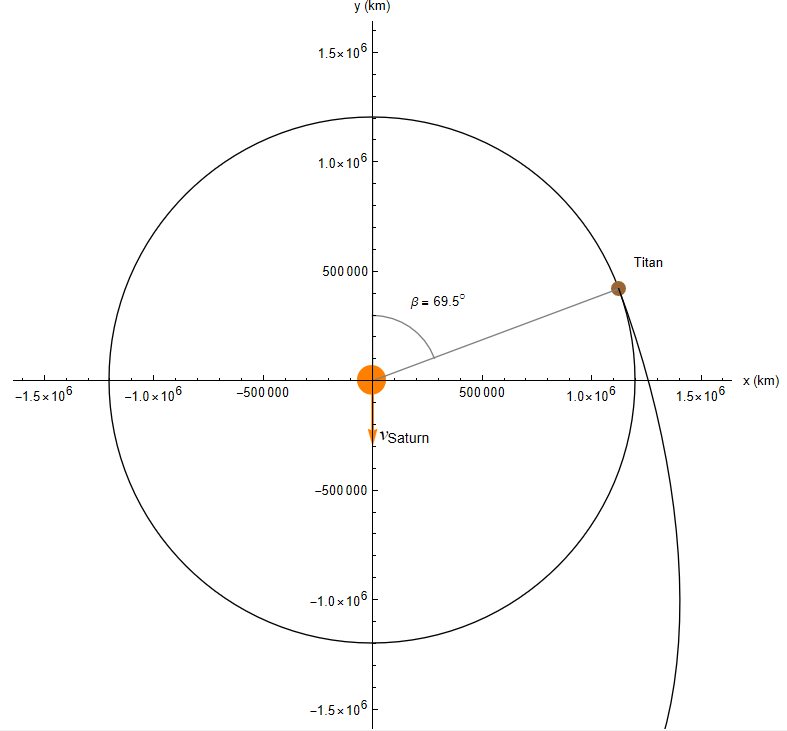
\includegraphics[width=7.5cm]{Project Figure 3.png}
    \caption{Titan(Brown) in circular orbit around Saturn(Orange) with arrival angle $\beta$ and hyperbolic trajectory of incoming spacecraft.}
\end{figure}
%%%%%%%%%%%%%%%%%%%%%%%%%%%%%%%%%%%%%%%%%%%%%%%%%%%%%%%%%%%%%%%%%%%%%%%%%%%%%%%%%%%%%%%%%%%%%%%%%%%%%%%%%%%%%%%%%%%%%%%%%

%%%%%%%%%%%%%%%%%%%%%%%%%%%%%%%%%%%%%%%%%%%%%%%%%%%%%%%%%%%%%%%%%%%%%%%%%%%%%%%%%%%%%%%%%%%%%%%%%%%%%%%%%%%%%%%%%%%%%%%%%%%%
\subsubsection{Titan Aerocapture}

At arrival, the spacecraft will be traveling at 9.63343 km/s with respect to Saturn as found in (17). Titan orbits Saturn at a velocity of 5.62222 km/s as found in (18). From this, we concluded in (19) that another burn of 4.01121 km/s was necessary to slow down and match Titan's velocity before landing there. This value represents the relative velocity between Titan and the spacecraft since both have parallel velocity vectors at perigee. Rather than slowing the spacecraft via propellant, we consider taking advantage of Titan's thick atmosphere by slowing down via aerobraking.\par

The atmosphere on Titan extends outward 600km from it's surface, about 10 times higher than that of Earth\cite{NASA} With a suitable heat shield, a spacecraft can not only slow to a captured orbit around Titan, but fall through the atmosphere directly to landing. This method was used by the Huygens probe that was carried to Titan via NASA's Cassini mission, and is still the only craft to have landed there. The probe entered Titan's atmosphere at about\cite{Springer}{6 km/s}, eventually landing using a heat shield and parachute. After descending through the atmosphere for over 2 hours, it impacted the surface at a velocity of only{5 m/s}\cite{Educational}. \par

Our spacecraft would only have a velocity of just over 4 km/s with respect to Titan upon entering it's atmosphere, which is a reasonable value compared to the Huygens probe. With a suitable heat shield and parachute, our craft will use this same technique to land safely on Titan's surface. The total $\Delta v$ for our mission design will primarily consist of the first burn to leave parking orbit around Earth as calculated in (14), neglecting $\Delta v$ required to slow down at Titan's orbit, giving

\begin{equation}
\Delta \!\ v_{\infty \text{tot}} = \Delta \!\ v_{\infty 1} + 0 = 7.28358 \ km/s.
\end{equation}

This is a great improvement to the $\Delta v$ budget, and cuts the mass required for propellant by roughly 35\%. This significant improvement comes at the small cost of added weight from both the heat shield and parachute. Additionally, this theoretical calculation of $\Delta v$ will not be the exact number that the mission plans for. It is still important to consider room for error with the initial launch and transfer burn, so a small amount of extra propellant will be added in order to account for any necessary correction burns throughout the mission. 
%%%%%%%%%%%%%%%%%%%%%%%%%%%%%%%%%%%%%%%%%%%%%%%%%%%%%%%%%%%%%%%%%%%%%%%%%%%%%%%%%%%%%%%%%%%%%%%%%%%%%%%%%%%%%%%%%%%%%%%%%%%%

\section{Propulsion}
\subsection{Introduction}
\par The propulsion system is a critical component of a space mission as it provides the necessary thrust to achieve the required velocity for transferring, controls the spacecraft's weight with propellant and performs mid-flight corrections. When selecting a propulsion system, several factors must be considered, including the engine type, propellant type, and propellant mass.\\
\par The engine type is the most crucial factor since it determines the spacecraft's speed, trajectory, and maneuverability. Liquid propellants are more commonly used since they provide more efficient combustion and can be throttled to adjust the engine's thrust. Propellant mass depends on the mission's requirements and the engine's efficiency.\\
\par In this project, the spacecraft will travel from Earth's low orbit to Titan, Saturn's moon. Therefore, thrust, specific impulse, safety, temperature, and payload are crucial factors to consider. The propulsion system must be designed to support the weight and size of the spacecraft and any scientific instruments or equipment carried onboard. Also, SpaceX has capabilities to provide the departure $\Delta v$ for this mission\cite{taylor_2015}. Hence, the main propulsion system will focus on the in-space propulsion system. The propulsion system may be required with minimal components and propellants as the plan described in the Astrodynamics section of Titan Aerocapture. However, in the event of a change in the plan, the fuel and engines will be prepared for both scenarios.
\subsection{Propellant}
\par The time of flight from Earth to Saturn is approximately 6 years, and potentially longer for another transfer to be captured in Titan's atmosphere. As a result, the propellant used in the spacecraft's propulsion system must be able to be stored for extended periods and reignite to be captured in Saturn's orbit.\\
\par Hypergolic propellants are the most suitable type of propellant for this mission. Hydrazine and dinitrogen tetroxide (NTO) are excellent choices for propellants in this space mission due to their high-energy output and ability to be stored for long periods without degradation. These bipropellants offer exceptional performance, allowing the spacecraft to achieve the required velocity $\Delta v$ to be captured by Saturn and Titan. Their high specific impulse enables the spacecraft to cover greater distances with less fuel, reducing the overall weight of the spacecraft and, therefore, the cost of the mission. Additionally, since they are hypergolic, the propellants ignite instantly on contact, making the engine's start-up and operation more reliable and efficient. \cite{braeunig_2008}
\subsection{Engine}
\par The selection of engines with reasonable specific impulse and thrust capability is crucial to the success of a space mission. As mentioned earlier, a higher specific impulse means higher efficiency in producing more thrust for the same amount of propellant or a lower mass of propellants. This translates to reduced propellant costs and greater mission flexibility.\\
\par For the purpose of achieving the necessary $\Delta v$ to be captured in Saturn's orbit, the R-42DM 890N (200 lbs) Dual Mode High-Performance Rocket Engine from Aerojet Rocketdyne was selected as the main engine for the mission. This bipropellant rocket engine has the capability to provide the required thrust for the mission and has a specific impulse of 327 seconds, which ensures efficient use of propellant. \cite{wilson_2020}\\



{\centering
\begin{tabular}{ |p{4cm}||p{4cm}|  }
\hline
\multicolumn{2}{|c|}{R-42DM 890N\cite{wilson_2020}}\\
 \hline
 \multicolumn{2}{|c|}{Characteristics} \\
 \hline
 Propellant&Hydrazine/NTO (MON-3)\\
 \hline
 Expansion Ratio&200\\
 \hline
 Oxidizer / Fuel Ratio&1\\
 \hline
 Flowrate (g/s)&277\\
 \hline
 Mass (kg)&7.3\\
 \hline
 Outlet Diameter (mm)&381\\
 \hline
 \multicolumn{2}{|c|}{Performance} \\
 \hline
 Specific Impulse (s)&327\\
 \hline
 Thrust (N)&890\\
 \hline

\end{tabular}
\par}

\begin{figure}[h!]
    \centering
    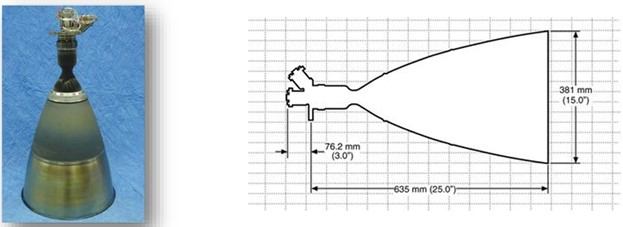
\includegraphics{Kims Pic 1.jpg}
    \caption{Figure : R-42DM 890N \cite{wilson_2020}}
    \label{fig:my_label}
\end{figure}

\par However, mid-course corrections are also critical for ensuring that the spacecraft stays on its intended trajectory toward its destination. As the change of $\Delta v$ required for mid-course correction is smaller than that required $\Delta v$ for capture, a smaller and more capable thrust engine can be used for this purpose\cite{burk_2005}. The MRM-122 130N (30-lbf) Rocket Engine Module from Aerojet Rocketdyne was selected as the secondary engine for mid-course corrections. It is a monopropellant rocket engine with a specific impulse of 228 seconds, which is efficient in terms of propellant consumption and capable of providing the necessary maneuver changes. \cite{wilson_2020}

{\centering
\begin{tabular}{ |p{4cm}||p{4cm}|  }
\hline
\multicolumn{2}{|c|}{MRM-122 130N (30-lbf) Rocket Engine Module\cite{wilson_2020}}\\
 \hline
 \multicolumn{2}{|c|}{Characteristics} \\
 \hline
 Propellant&Hydrazine\\
 \hline
 Expansion Ratio&20.7\\
 \hline
 Flowrate (g/s)&24-63.5\\
 \hline
 Mass (kg)&0.66\\
 \hline
 Outlet Diameter (mm)&57\\
 \hline
 \multicolumn{2}{|c|}{Performance} \\
 \hline
 Specific Impulse (s)&228\\
 \hline
 Thrust (N)&51-142\\
 \hline

\end{tabular}
\par}
\begin{figure}[h!]
    \centering
    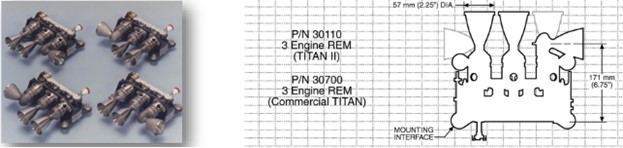
\includegraphics{Kims Pic 2.jpg}
    \caption{Figure : R-42DM 890N (Wilson, 2020)}
    \label{fig:my_label}
\end{figure}

\par To summarize, the plan for capturing in Saturn's orbit with the application of $\Delta v$ and arriving at Titan involves using a high-performance main engine along with a smaller engine for mid-course corrections. On the other hand, the plan for aerocapture to Titan only requires the use of the mid-course correction engine for the mission

\subsection{Payload}
\par The values for the payload have been assumed and approximated from past missions and other component data. The main parts of the payload are the Rover and Satellite. The landing equipment includes the heat shield, parachute, and other structural parts necessary for the safe landing of the rover. The structure consists of the decoupling unit for the satellite, as well as other structural connections for the propulsion and communication systems. The propulsion system consists of the engines, fuel tanks, valves, and other equipment needed for propulsion, excluding the propellants. The Comm. system allows for communication between the main spacecraft and the ground command but does not include the satellite's communication system.\\

{\begin{center}

\begin{tabular}{ |p{4cm}||p{2cm}|  }
 \hline
 \multicolumn{2}{|c|}{Payload of the Mission} \\
 \hline
 \hline
 Components&Mass\\
 \hline
 Rover (kg)&900\\
 \hline
 Landing Equipment (kg)&225\\
 \hline
 Satellite (kg)&730\\
 \hline
 Structure (kg)&225\\
 \hline
 Propulsion System (kg)&150\\
 \hline
 Comm. System (kg)&150\\
 \hline

\end{tabular}
\end{center}
\\

\subsection{Propellant Mass}
\par For the calculation of the required propellants, we estimate the mid-course correction $\Delta v$ from the past missions and approximations. The altitude of the parking orbit is an additional 1000 km from Titan's orbit. Cassini Mission’s estimated mid-course correction $\Delta v$ was about 1 km/s as total adjustments\cite{goodson_gray_hahn_peralta_1998}. Hence, total $\Delta v$ is calculated by adding capture $\Delta v_{c}$, transfer $\Delta v_{t}$ at Saturn’s orbit, and mid-course correction $\Delta v_{MCC}$. The $\Delta v$s are $\Delta v_{c} = 4.01121 \ km/s$ and $\Delta v_{MCC} = 1 \ km/s$.
 



\begin{equation}
\Delta v = \Delta v_{c}+ \Delta v_{MCC} = 5.0112 \ km/s  
\end{equation}
   


\par 
 Specific impulse, $I_{sp}$ is based on the main engine’s performance which is 327 seconds. 
Gravity $g_{0}$ is 9.81 meters per second.
The ideal rocket equation\cite{curtis_2020} is\\

\begin{equation}
\Delta v = I_{sp}g_{0}ln(\frac{\Delta m}{m_t})    
\end{equation}



 \par 
From the ideal rocket equation, the mass ratio can be calculated.
\begin{equation}
\frac{\Delta m}{m_t} = 1 - exp( \frac{-\Delta v}{ I_{sp}g_{0}}) = 0.7903 
\end{equation}


Once the mass ratio is calculated, the total mass of the spacecraft is
\begin{equation}
m_{t}=\frac{m_{P}}{1-\frac{\Delta m}{m_{t}}} = 11,350.5  \ kg    
\end{equation}
 

Hence, the propellant mass is
\begin{equation}
\Delta m = m_{t}-m_{P} = 8,970.5 \ kg 
\end{equation}

\par Therefore, 8,970.5 kg of hydrazine and dinitrogen tetroxide is needed. Since the main engine’s oxidizer and fuel ratio is 1, each of these is 4,485.25 kg for capturing in Saturn's orbit with the application of $\Delta v$ and arriving at Titan.\\
\par By using the same equations from $(22)$ to $(26)$ with $I_{sp}=228 s$ and $\Delta v = 1 km/s$ (since only $\Detla v_{MCC}$ will be used), the total mass of the spacecraft is $m_{t}=3,721.74 kg$. Therefore, 1,341.74 kg of hydrazine is needed for the aerocapture of Titan.



\subsection{Compare with Cassini}
\par The Cassini-Huygens mission was an ambitious and complex mission that required careful planning and execution. One of the key components of the mission was the propulsion system, which included two different types of engines and a number of thrusters for attitude control and small maneuvers. The main engine, which was used for spacecraft velocity and trajectory correction changes, was a critical component of the propulsion system. To ensure redundancy and minimize the risk of failure, there were two identical main engines on board: one was in use and the other served as a backup. This approach ensured that the spacecraft had a backup engine in case the primary one malfunctioned or failed. In addition to the main engines, there were also 16 monopropellant hydrazine thrusters on board, eight of which were prime and eight were backups. These thrusters were used for attitude control and small velocity-change maneuvers and provided additional redundancy to the propulsion system\cite{isbell_savage_o’donnell_murrill_diller_1997}. The main engine used in the Cassini-Huygens mission had a specific impulse of 312 seconds, which is a measure of the efficiency of the engine\cite{bailey_2018}.\\

\par The total mass of the Cassini-Huygens spacecraft was known from the data. The Cassini orbiter, which was the primary spacecraft, had a mass of 2,125 kg. When the mass of the Huygens lander, the launch vehicle, and 3,267 kg of propellants were added, the total mass of the spacecraft was 5,712 kg \cite{mahaffy_2004}.\\

\par For comparison purposes, it was assumed that all of the propellants on board had been used once the spacecraft arrived at Titan. However, it should be noted that the spacecraft contained enough propellants to perform further missions until the Grand Finale.\\
\par Based on these data and assumptions, the total $\Delta v$ (change in velocity) required for the Cassini-Huygens mission was estimated to be 3.0264 km/s, which was 1.985 km/s less than the plan of capturing in Saturn's orbit with the application of $\Delta v$ and arriving at Titan. Also, the total mass of propellants required was about 5,700 kg less than the following plan, due to the use of swing-by maneuvers to minimize the $\Delta v$ and propellant requirements. However, the plan of the aerocapture of Titan has opposite results. The total $\Delta v$ of this plan was 2.0264 km/s less and 1,925 kg of propellants was less than the Cassini -Huygens mission.




\section{Payload, Power, Electrical}
\par There are two major areas for the electronics of our project, the rover that will be left on Titan and the satellite that will be left orbiting Titan. The rover is based on the Curiosity rover, and the satellite is based on the Voyager probe. This was done because there are no extensive breakdowns of the mass and power consumption of the equipment on the Curiosity rover or the Voyager probe. Upon approval of the proposal, the electronics will be tailored to work best in the conditions they will be in, similar to how the Mars rover was designed.\\
\par Our rover is copies the Curiosity Rover since the mission that it was designed for is very similar to our mission. The major areas of electronics are: Electrical Power, Communications, Sensors, and Mechanics. The rover also has wheels to allow it to move, and a robotic arm to interact with the environment. The power for the rover will come from one Multi-Mission RTG or MMRTG, as well as two lithium-ion batteries to supplement its power when our draw exceeds the power output of the rover’s reactor\cite{NASA-Power}. Radioisotope thermoelectric generators use heat generated by nuclear materials, usually Plutonium, to generate power. They do this using thermoelectric materials. When a voltage is placed across a thermoelectric material one side will heat up and the other will cool down. RTG’s instead uses the heat put off by the nuclear material and the cooler temperature of the atmosphere to generate power\cite{NASA-Resources}.  There are several sensors on the rover, a few are listed here: Hazcams, Navcams, Mastcam, Chemcam, MAHLI, MARDI\cite{NASA-Resources}. The Hazcams and Navcams are camera systems the rover uses to navigate and detect and avoid hazards\cite{NASA-Cameras}. The Mastcam is mounted on the mast and takes both color pictures and videos of the planet\cite{NASA-Cameras}. The Chemcam analyzes what the soil and rock are made of. It does this with a spectrometer and a laser system\cite{NASA-Cameras}. The Mars Hand Lens Imager or MAHLI is a camera mounted on the hand of the rover and it takes photos on the scale of 12.5 microns of rocks and minerals\cite{NASA-Cameras}. The Mars Decent Imager or MARDI is mainly used during landing once the heatshield is gone, it can send four frames per second of high-resolution video\cite{NASA-Cameras}. Communicating with the rover is critical which is why the rover has three separate antennas\cite{NASA-Communications}. The first antenna is the Ultra-High Frequency or UHF antenna which uses frequencies in the range of 400 Megahertz and can transmit two megabits per second\cite{NASA-Communications}. Next is the X-Band High Gain antenna is a “steerable” antenna, it can transmit more than 800 bits per second since we will be using the Deep Space Network\cite{NASA-Communications}. The last antenna is the X-Band Low Gain antenna is an Omnidirectional antenna, which means it can receive data from all directions, it is mainly used for receiving data\cite{NASA-Communications}. The X-Band low gain antenna can transmit at a rate of Eight Gigahertz \cite{NASA-Communications}. X-band is between eight and twelve Gigahertz, x-band is a fancy name for this range\cite{NASA-Basics_of_Space_Flight}.\\
\par For the satellite we used Voyager as the example mission. This is because 50 years later the probe is still communicating. Also, if the communications equipment for the voyager probe can communicate with Earth from outside of the solar system, then it will be able to relay information to Earth from Titan. The Voyager probe had several sensors and lenses in addition to its communication equipment. These are stripped away for this mission and will be replaced with additional fuel to help keep it in the correct orbit around Titan. The satellite will be powered by three RTG’s\cite{NASA-NSSDCA}. These are similar to the MMRTG on the rover by more powerful, they put out 470 Watts as opposed to the MMRTG’s 110 Watts\cite{NASA-NSSDCA}). As for the communication equipment, the satellite will use a high gain antenna that can use both X-band and S-band, it also has a low gain antenna as a backup \cite{NASA-NSSDCA}. The S-band is roughly between two and four Gigahertz \cite{NASA-Basics_of_Space_Flight}. A high gain antenna and a low gain antenna differ in the area they output signal. High gain antennas transmit data in a cone, this cone is narrower than with the low gain antenna\cite{ESA}. This means that the signal from the low gain antenna is easier to “see” but is weaker. Whereas the signal from the high gain antenna is stronger but requires a more precise aiming\cite{ESA}. 



\section{Budget}
\par The main costs of the propulsion system are propellants and rocket engines. According to the Department of Defense Fiscal Year 2023, the cost of propellants for their customers is as follows: hydrazine is priced at \$151.70 per pound, and nitrogen tetroxide (NTO) MON-3 is priced at \$151.00 per pound \cite{sninsky_2022}. Based on these prices, the required amounts of 4,489.39 kg (9,897.41 lb) for hydrazine and NTO MON-3 respectively, result in a cost of \$1,501,436.30 for hydrazine and \$1,494,508.11 for NTO MON-3.\\
\par The main engine and sub-engine costs are estimated from similar types of engines since the prices were not available in the catalog. R-4D is a hypergolic engine with a 490 N thrust power and the price was approximately \$30,000 in 1960, which would be equivalent to around \$255,000 in 2021 after adjusting for inflation \cite{fisher_rahman_2009}. Hence, the modern price is estimated to be around \$300,000. The R-42DM engine provides roughly twice the thrust power of the R-4D engine and the MRM-122 engine provides about one-fourth of the thrust power of the R-4D engine. Thus, the estimated cost for both engines is \$600,000.\\
\par The total cost of the propulsion system would therefore be \$3.6 million.\\

\par We estimate the cost of the payload, power, and electrical to be on the low end similar to they Voyager 1 and 2 missions.  They contained similar equipment and purposes as our mission.  This includes the spacecraft development, launch, and mission operations.  The Voyager mission cost approximately \$865 million.Voyager also had an additional \$30 million to run its VIM for an additional 2 years. \cite{Voyager}
 Since we are landing the rover on Titan and will have a satellite orbiting Saturn we expect the budget to be similar.\\  
 \par On the high end of the budget cost, we modeled our launch to be similar to the curiousity mission.  The curiosity mission cost \$2.42 billion for the development and launch and an additional \$116 million for the rover to operate on the surface of Mars.  The titan mission is very similar to the Mars mission so we can estimate on the upper end, for our mission to be similar to the curiosity mission. \cite{Curiosity}


\section{Conclusion}
In conclusion, we believe a mission to Titan will develop our overall knowledge and understanding of our own planet.  We believe that it will advance the human understanding of events in our solar system.  The benefits of the mission are worth the cost to get us to Titan.  Overall we believe this is a worthwhile endeavor to benefit the future of mankind.


\bibliography{sample}

\end{document}
